\documentclass[a4paper,10pt]{article}
\usepackage[a4paper,top=24mm,bottom=25mm,left=23mm,right=23mm,headheight=15pt]{geometry}
\usepackage{fontspec}
\usepackage{amsmath,amssymb,mathtools}
\usepackage{unicode-math}
\usepackage{graphicx}
\usepackage{booktabs}
\usepackage{fancyhdr}
\usepackage{titlesec}
\usepackage[hidelinks]{hyperref}
\usepackage{microtype}

\setmainfont{Times New Roman}
\setmathfont{STIX Two Math}
\setmonofont{Menlo}
\setlength{\parindent}{1.5em}
\setlength{\parskip}{0.2em}
\setlength{\emergencystretch}{3em}
\linespread{1.0}
\allowdisplaybreaks[2]

\titleformat{\section}{\Large\bfseries}{\thesection}{0.7em}{}
\titleformat{\subsection}{\large\bfseries}{}{0pt}{}
\titlespacing*{\section}{0pt}{2.2ex plus 0.5ex}{0.9ex}
\titlespacing*{\subsection}{0pt}{1.8ex plus 0.4ex}{0.7ex}
\pagestyle{fancy}
\fancyhf{}
\fancyhead[L]{\small CS224N \textbar{} Assignment 3}
\fancyhead[R]{\small Selene's Blog}
\fancyfoot[C]{\small\thepage}
\renewcommand{\headrulewidth}{0.4pt}
\hypersetup{pdftitle={CS224N | Assignment 3},pdfauthor={Selene}}

\begin{document}
\begin{center}
  {\Large\bfseries CS224N \textbar{} Assignment 3\par}
  \vspace{0.5em}
  Selene \quad\textperiodcentered\quad October 1, 2026
\end{center}
\vspace{0.7em}

\section{Problem 1}

\subsection{(a)}
\noindent\textbf{1.} Make \(k_j^\top q\) much larger than every other \(k_i^\top q\).

\noindent\textbf{2.} The output is approximately \(v_j\).

\subsection{(b)}
Let \(q=\lambda(k_a+k_b)\), where \(\lambda\) is a sufficiently large positive number. Since the keys are pairwise orthogonal unit vectors,
\[
k_a^\top q=k_b^\top q=\lambda.
\]
For every \(i\ne a,b\), we also have \(k_i^\top q=0\). Thus the softmax scores of \(k_a\) and \(k_b\) are both \(e^\lambda\), while every other score is \(e^0\). When \(\lambda\) is large, the contributions of the other keys become negligible, so
\[
c=\sum_i\alpha_i v_i\approx\frac{1}{2}(v_a+v_b).
\]

\subsection{(c)}
\noindent\textbf{1.} The idea is the same as in (b), except that we use the mean of each key distribution rather than a particular sampled key. The perturbations are small, so the relevant keys remain close to \(\mu_a\) and \(\mu_b\).

\noindent\textbf{2.} Here \(k_a\) varies substantially in length along the direction of \(\mu_a\). Write \(k_a\approx s\mu_a\), where \(s\) fluctuates considerably. Then \(k_a^\top q\approx\lambda s\), whereas the length of \(k_b\) is relatively stable and \(k_b^\top q\approx\lambda\). Consequently, the attention output \(c\) shifts between \(v_a\) and \(v_b\). In the first case its variance is small and the output is stable; in this case its variance is larger.

\subsection{(d)}
\noindent\textbf{1.} Unlike (c), where one head uses a single query to attend to both \(a\) and \(b\), the two heads now divide the work. The means \(\mu_i\) are pairwise orthogonal and the key perturbations are small, so \(q_1\) has a large dot product only with \(k_a\), giving \(c_1\approx v_a\). Similarly, \(c_2\approx v_b\). Therefore,
\[
c=\frac{1}{2}(c_1+c_2)\approx\frac{1}{2}(v_a+v_b).
\]

\noindent\textbf{2.} This is the multi-head counterpart of (c)(ii). Changes in the length of \(k_a\) make \(k_a^\top q_1\) fluctuate, so \(c_1\) has relatively high variance: when \(k_a\) is long, \(c_1\approx v_a\), and when it is short, the attention paid to \(v_a\) weakens. But \(q_2\perp\mu_a\), so variation in \(k_a\) along \(\mu_a\) has almost no effect on the second head. We still have \(c_2\approx v_b\) with low variance. Hence
\[
c=\frac{1}{2}(c_1+c_2).
\]
Only the first head's output fluctuates; the second remains stable. In the single-head attention of (c)(ii), the weights on both \(v_a\) and \(v_b\) fluctuate together. Averaging the two heads therefore gives an output with lower variance.

\subsection{(e)}
Multi-head attention splits a task that one head would otherwise perform alone: one head attends to \(v_a\), and another attends to \(v_b\). A fluctuation in the length of one key mainly affects its corresponding head, while the other head remains stable. Averaging the head outputs reduces the variance of the final result and makes attention more robust.

\section{Problem 2}

\subsection{(a)}
\noindent\textbf{1.} From \(X_{\mathrm{perm}}=PX\), we obtain \(Q_{\mathrm{perm}}=PQ\), \(K_{\mathrm{perm}}=PK\), and \(V_{\mathrm{perm}}=PV\). Therefore,
\[
\frac{Q_{\mathrm{perm}}K_{\mathrm{perm}}^\top}{\sqrt d}
=P\frac{QK^\top}{\sqrt d}P^\top.
\]
Using the stated property of row-wise softmax and \(P^\top P=I\),
\[
\begin{aligned}
H_{\mathrm{perm}}
&=\operatorname{softmax}\left(P\frac{QK^\top}{\sqrt d}P^\top\right)PV \\
&=P\operatorname{softmax}\left(\frac{QK^\top}{\sqrt d}\right)P^\top PV \\
&=PH.
\end{aligned}
\]
Since \(P\mathbf{1}=\mathbf{1}\), it follows that
\[
\begin{aligned}
Z_{\mathrm{perm}}
&=\operatorname{ReLU}(PHW_1+\mathbf{1}b_1)W_2+\mathbf{1}b_2 \\
&=\operatorname{ReLU}\left(P(HW_1+\mathbf{1}b_1)\right)W_2+P\mathbf{1}b_2 \\
&=P\operatorname{ReLU}(HW_1+\mathbf{1}b_1)W_2+P\mathbf{1}b_2 \\
&=PZ.
\end{aligned}
\]
\noindent\textbf{2.} Without positional embeddings, the Transformer is permutation-equivariant: \(Z_{\mathrm{perm}}=PZ\). It cannot tell where a token originally appeared. Because the meaning of text depends on word order, positional embeddings are needed to supply position information.

\subsection{(b)}
\noindent\textbf{1.} Yes. With positional embeddings, \(X_{\mathrm{pos}}=X+\Phi\). If the tokens are permuted while their positions stay fixed, the new input is \(X_{\mathrm{perm,pos}}=PX+\Phi\). Permuting the original full input instead would give \(P(X+\Phi)=PX+P\Phi\). These expressions generally differ, so different word orders produce different input representations. The Transformer can use the position assigned to each token to recover order information.

\noindent\textbf{2.} No, for the sinusoidal embeddings in the question. If distinct integer positions \(t\ne s\) had identical embeddings, their first two coordinates would require \(\sin t=\sin s\) and \(\cos t=\cos s\). This implies \(t=s+2\pi k\) for some integer \(k\). Since \(t-s\) is an integer and \(2\pi k\) can be an integer only when \(k=0\), we must have \(t=s\), a contradiction.

\section{Problem 3}

\subsection{(a)}
This problem implements a decoder-only, GPT-2-style Transformer.

\noindent\textbf{MLP.} The MLP independently applies two linear transformations to each token, with GELU between them:
\[
\operatorname{MLP}(x)=W_2\operatorname{GELU}(W_1x+b_1)+b_2.
\]
The first layer expands the hidden dimension from \(d_{\text{model}}\) to \(4d_{\text{model}}\); the second projects it back to \(d_{\text{model}}\).

\noindent\textbf{CausalAttention.} First obtain \(Q\), \(K\), and \(V\) from the input, then compute scaled dot-product attention:
\[
\operatorname{Attention}(Q,K,V)=
\operatorname{softmax}\left(\frac{QK^\top}{\sqrt{d_h}}+M\right)V.
\]
Here \(M\) is a causal mask that permits the lower triangular part of the score matrix. Position \(t\) can attend only to positions \(0,\ldots,t\). Setting the scores for future positions to \(-\infty\) makes their softmax weights zero. For multi-head attention, reshape \([B,T,d_{\text{model}}]\) into \([B,h,T,d_h]\), compute attention separately for each head, and concatenate the results.

\noindent\textbf{DecoderBlock.} This implementation uses Pre-LN: apply layer normalization before attention and the MLP, then add each sublayer's residual connection:
\[
\begin{aligned}
H &= X+\operatorname{CausalAttention}(\operatorname{LN}_1(X)),\\
Y &= H+\operatorname{MLP}(\operatorname{LN}_2(H)).
\end{aligned}
\]

\noindent\textbf{Transformer.} Add token and position embeddings, pass the result through the decoder blocks, then apply a final layer normalization and the language-model head to obtain logits:
\[
H^{(0)}=E_{\text{token}}(x)+E_{\text{position}}(0,\ldots,T-1),
\]
\[
\operatorname{logits}=H^{(L)}W_{\text{lm}}^\top.
\]
At each generation step, take the token with the largest logit at the final position:
\[
x_{\text{next}}=\arg\max_v\operatorname{logits}_{-1,v}.
\]
Append that token to the input and repeat. If the sequence exceeds the context length, keep only the most recent \texttt{context\_length} tokens for the forward pass.

\subsection{(b) Training the Transformer}
\texttt{get\_loss\_on\_batch} uses next-token prediction. Given an input sequence
\[
(x_0,x_1,\ldots,x_{T-1}),
\]
the logits at position \(t\) predict \(x_{t+1}\). Thus we remove the final logit position and the first label token:
\[
\operatorname{loss}=
\operatorname{CrossEntropy}\left(
\operatorname{logits}_{[:,0:T-1,:]},
x_{[:,1:T]}
\right).
\]
In the implementation, flatten the batch and sequence dimensions before passing them to \texttt{F.cross\_entropy}. The final position has no next token, so it does not contribute to the loss.

After 100 batches, the loss decreases overall from about \(10.83\) to about \(10.77\), showing that the model has begun to learn from the data. The gradient norm stays within a modest range, with no obvious gradient explosion.

\begin{figure}[htbp]
  \centering
  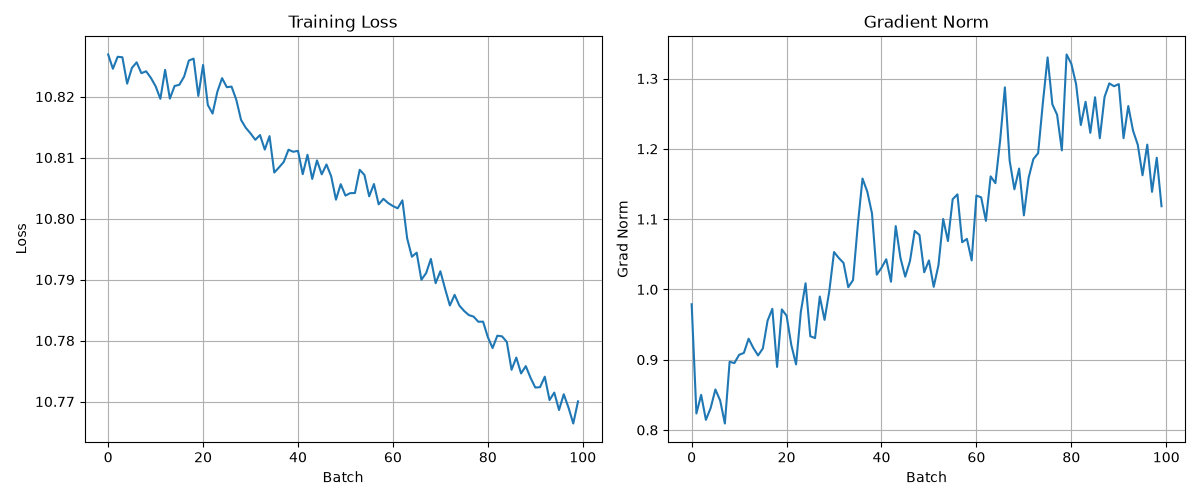
\includegraphics[width=0.76\linewidth]{../../assets/img/posts/cs224n-assignment-3/losses-and-grad-norms.png}
  \caption{Training loss and gradient norm over 100 batches.}
\end{figure}

\subsection{(c) Bonus: Faster Training}
With the number of training steps fixed at 100, the goal is to obtain a lower final loss than the baseline under the same budget. I applied three changes in sequence: a higher learning rate, no weight decay, and a learnable bias in the language-model head.

\begin{center}
\begin{tabular}{lr}
\toprule
Setting & Final loss after 100 steps \\
\midrule
Baseline & \(\approx 10.77\) \\
Learning rate: \(10^{-3}\) & \(6.449274\) \\
+ No weight decay & \(6.446831\) \\
+ LM head bias & \(\mathbf{6.427308}\) \\
\bottomrule
\end{tabular}
\end{center}

Increasing the learning rate produces the largest improvement in convergence over the fixed number of steps. Removing weight decay slightly improves the training loss under this budget; the LM-head bias can directly learn an overall frequency offset for each token and reduces the final loss further.

\end{document}
